\subsection{Gekrümmte Kanten}

Wir haben gesehen, dass für Polyeder mit gewissen Symmetrieeigenschaften die Summe der quadrierten projizierten Kantenlängen unter Orthogonalabbildungen unabhängig ist von der Ebene, auf die projiziert wird. Andererseits haben wir auch gesehen, dass die Symmetrieeigenschaften zwar hinreichend, aber nicht notwendig sind. Eine weitere naheliegende Frage ist, ob dies auch für gekrümmte Linien gilt. Dafür betrachten wir die Projektion eines regulären Oktaeders $O$ auf eine Kugeloberfläche, siehe Abbildung \ref{fig:oktaederprojiziertaufKugel}.

\begin{figure}[htp]
    \centering
    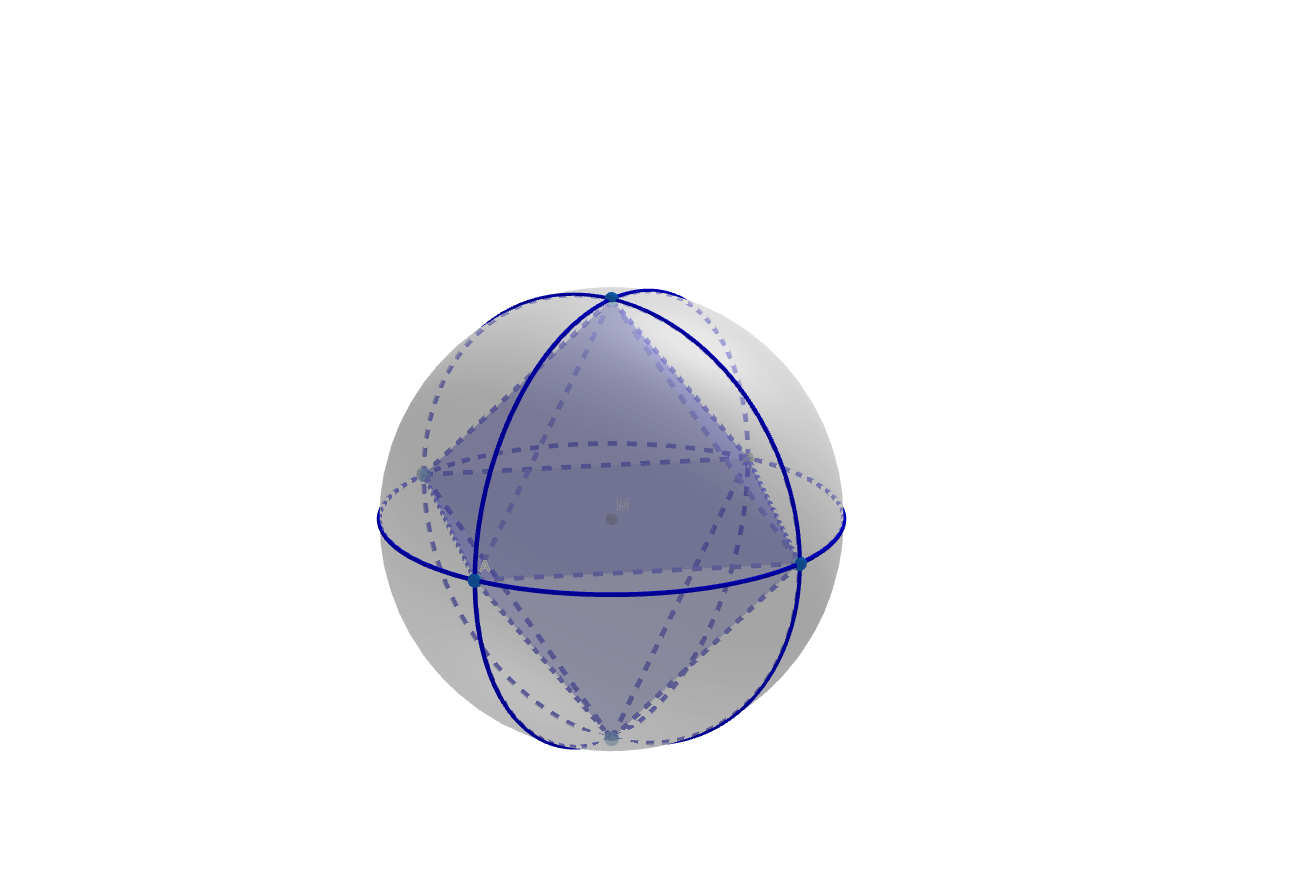
\includegraphics[width=10cm]{images/gekrümmteKanten/oktaederprojiziertKugel.png}
    \caption{Projektion eines regulären Oktaeders auf eine Kugeloberfläche.}
    \label{fig:oktaederprojiziertaufKugel}
\end{figure}

Die Projektion $P_O$ des regulären Oktaeders auf die Kugeloberfläche besteht aus drei orthogonalen Großkreisen und teilt die Kugeloberfläche in 8 sphärische Dreiecke ein. Die Symmetrieeigenschaften des euklidischen Oktaeders bleiben dabei erhalten, d.\,h. die Projektion $P_O$ besitzt weiterhin die volle Oktaedersymmetrie $H$. Wir betrachten nun die Orthogonalprojektion auf die Ebenen
\begin{align}
    E_1 &: z=0 \nonumber \\
    E_2 &: x-y=0. \nonumber
\end{align}
Die Projektionen $\Pi_{E_1}$ und $\Pi_{E_2}$ sind in Abbildung \ref{fig:oktaedersichten} visualisiert.

\begin{figure}[htbp]
     \centering
     \begin{subfigure}[b]{0.45\textwidth}
         \centering
         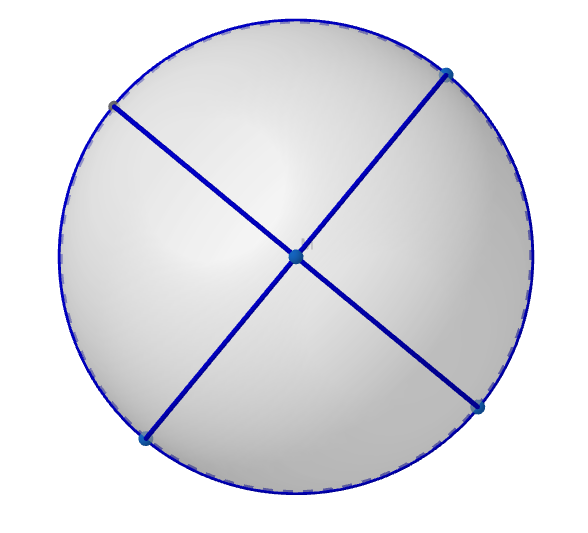
\includegraphics[width=\textwidth]{images/gekrümmteKanten/oktaederprojiziertKugelSichtOben.png}
         \caption{Projektion von $P_O$ auf die Ebene $E_1$.}
         \label{fig:oktaederSichtoben}
     \end{subfigure}
     \hfill
     \begin{subfigure}[b]{0.45\textwidth}
         \centering
         \includegraphics[width=\textwidth]{images/gekrümmteKanten/oktaederprojiziertKugelSichtseitlich.png}
         \caption{Projektion von $P_O$ auf die Ebene $E_2$.}
         \label{fig:oktaederSichtseitlich}
     \end{subfigure}
        \caption{Projektion des Körpers $P_O$ auf die Ebenen $E_1$ und $E_2$.}
        \label{fig:oktaedersichten}
\end{figure}

Wir können nun die Summe der quadrierten Längen der projizierten Kurven ausrechnen. Sei $K_{P_O}$ die Menge der drei Großkreise und $d=2r$ der Kugeldurchmesser. Dabei ist zu beachten, dass ein orthogonal zur Projektionsebene stehender Großkreis in der Projektion als Strecke der Länge $d$ erscheint, diese Kurve jedoch doppelt durchlaufen wird (Vorder- und Rückseite der Kugel). Seine projizierte Bogenlänge beträgt folglich $2d$. Für die beiden Ebenen erhalten wir
\begin{align}
    \sum_{k \in K_{P_O}} \|\Pi_{E_1}(k)\|^2 &= (\pi d)^2 + (2d)^2 + (2d)^2 = \pi^2 d^2 + 2(2d)^2 \nonumber \\
    \sum_{k \in K_{P_O}} \|\Pi_{E_2}(k)\|^2 &= (2d)^2 + 2 \cdot l_{\text{Ellipse}}^2 = 4d^2 + 2 \cdot l_{\text{Ellipse}}^2 \nonumber
\end{align}
wobei $l_{\text{Ellipse}}$ der Umfang der projizierten Ellipsen in $E_2$ ist. Die Exzentrizität dieser Ellipsen entsteht durch die Projektion der Kreise unter einem Winkel von $45^\circ$. Ihre Halbachsen betragen somit $a = \frac{d}{2}$ und $b = \frac{d}{2\sqrt{2}}$. Da der Umfang einer Ellipse strikt durch die untere Schranke $l_{\text{Ellipse}} > \pi(a+b)$ abgeschätzt werden kann (vgl. \cite{almkvist1988gauss}), gilt:
\begin{align}
    l_{\text{Ellipse}} &> \pi \left( \frac{d}{2} + \frac{d}{2\sqrt{2}} \right) = \frac{\pi d}{2} \left( 1 + \frac{1}{\sqrt{2}} \right) \nonumber \\
    \implies 2 \cdot l_{\text{Ellipse}}^2 &> 2 \cdot \frac{\pi^2 d^2}{4} \left( 1 + \sqrt{2} + \frac{1}{2} \right) = \pi^2 d^2 \left( \frac{3}{4} + \frac{\sqrt{2}}{2} \right) > 1.45 \pi^2 d^2 . \nonumber
\end{align}
Vergleichen wir nun die Summen der beiden Projektionen, lässt sich die Ungleichung analytisch zeigen. Da $\pi^2 < 10$ und $1.45 \pi^2 \approx 14.3 > 14$ ist, gilt:
\begin{align}
    \sum_{k \in K_{P_O}} \|\Pi_{E_1}(k)\|^2 &= 8d^2 + \pi^2 d^2 \nonumber \\
    &< 18d^2 = (4 + 14) d^2 \nonumber \\ 
    &< 4d^2 + 1.45 \pi^2 d^2 \nonumber \\
    &< 4d^2 + 2 \cdot l_{\text{Ellipse}}^2 = \sum_{k \in K_{P_O}} \|\Pi_{E_2}(k)\|^2. \nonumber
\end{align}
Dies liefert den analytischen Beweis, dass die Konstanz der quadrierten Längen für sphärische Bögen nicht mehr gilt, da die Summe unter Variation der Projektionsebene eine strikte Ungleichung erfüllt.